\documentclass[border=2pt]{standalone}
\newcommand{\FontPath}{../../../../../../../assets/fonts/} 
\usepackage{fontspec}
\usepackage{unicode-math}

% Thiết lập phông chữ
\setmainfont{STIX Two Text}
\setsansfont{STIX Two Text}
\setmonofont{STIX Two Text}
\setmathfont{STIX Two Math}


\usepackage{xcolor}
\definecolor{quartoText}{RGB}{33, 37, 41} % Màu văn bản chính từ theme default của quarto
    
\usepackage{tikz}
\usetikzlibrary{arrows, positioning, calc}

% Đảm bảo mọi nội dung trong tikzpicture đều dùng màu văn bản chính
\AtBeginEnvironment{tikzpicture}{\color{quartoText}}
\usepackage{pgfplots}
\pgfplotsset{compat=1.18}
\usetikzlibrary{decorations.pathreplacing, calligraphy, intersections}
\usepgfplotslibrary{fillbetween}

\begin{document}
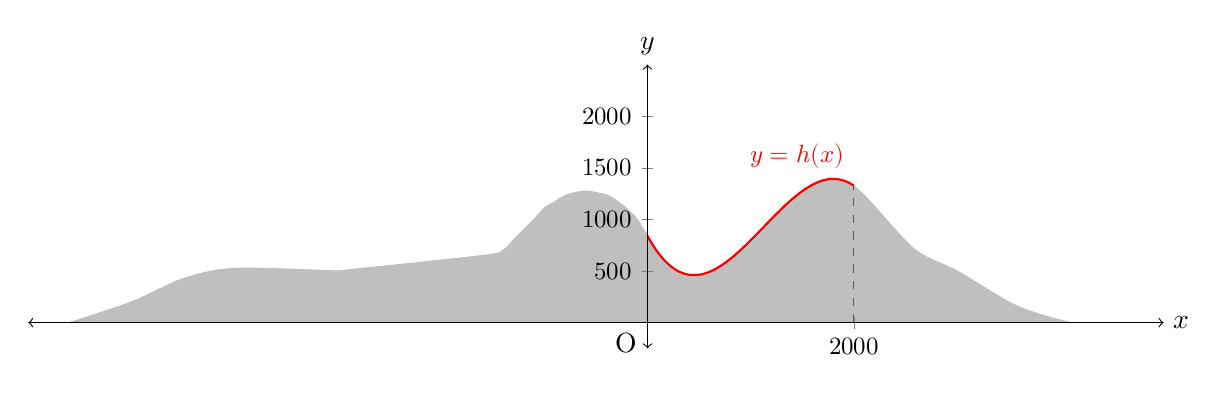
\begin{tikzpicture}
\begin{axis}[
    axis on top,
    axis lines=middle,
    axis line style={<->},
    xlabel={$x$},
    ylabel={$y$},
    xlabel style={at={(axis cs:5000,0)},anchor=west},
    ylabel style={at={(axis cs:0,2500)},anchor=south},
    xmin=-6000, xmax=5000,
    ymin=-250, ymax=2500,
    xtick={2000},
    ytick={500,1000,1500,2000},    
    tick label style={font=\small, /pgf/number format/use comma=false, /pgf/number format/1000 sep={}},
    axis equal image,
    width=16cm,
    height=8cm,
    clip=false,
    % scale only axis,
    % xscale=2,    
]

\addplot[
  name path=h,
  domain=0:2000, 
  samples=200, 
  restrict y to domain=-1000:3000,
  unbounded coords=discard, 
  thick, 
  red] 
{(-1/1320000)*x^3+(9/3520)*x^2-(81/44)*x+840};

% \addplot [
%   name path=baseline,
%   draw=none
% ] {0};

\path[name path=axis] (0,0) -- (2000,0);

\addplot [
  fill=lightgray,
  draw=none
] fill between [
  of=h and axis
];

\draw [dashed, opacity=.5] (2000,0) -- (2000,1325);

\node at (2000,1400) [anchor=south east, red] {\small $y=h(x)$};

\addplot [
  name path=h-1,
  lightgray,
  smooth
  ] coordinates {
  (2000,1325)
  (2100,1235) 
  (2200,1125) 
  (2600,700) 
  (3000,500)
  (3500,200)
  (3800,80)
  (4100,0)
  };

\path[name path=axis-1] (2000,0) -- (4100,0);

\addplot [
  fill=lightgray,
  draw=none
] fill between [
  of=h-1 and axis-1
];

\addplot[
    name path=h-2,
    smooth,
    lightgray
  ] coordinates {
    (0,840)
    (-100,1000)
    (-190,1095)
    (-270,1160)
    (-380,1230)
    (-500,1260)
    (-600,1275)
    (-700,1260)
    (-800,1230)
    (-900,1170)
    (-1000,1110)
    (-1100,1000)
    (-1200,900)
    (-1300,800)
    (-1400,700)
    (-1600,650)
    (-3000,500)
    (-3000,500)
    (-4000,525)
    (-4500,425)
    (-5000,200)
    (-5600,0)
  };

\path[name path=axis-2] (-5600,0) -- (0,0);

\addplot [
  fill=lightgray,
  draw=none
] fill between [
  of=h-2 and axis-2
];


\node at (axis cs:-10,-10) [anchor=north east] {O};
\end{axis}
\end{tikzpicture}
\end{document}
